\documentclass[12pt]{article}
\usepackage{amsmath, amsfonts}
\usepackage{graphicx}
\usepackage{tabularx}
\usepackage{epstopdf}
%\usepackage[dvips, final]{graphics}
%\DeclareGraphicsExtensions{.tif}
%\DeclareGraphicsRule{.tif}{eps}{.tif.bb}{`tiff2ps -e #1}
\graphicspath{{./img/}}
\usepackage[margin=1in]{geometry}

% Chinese name
\usepackage{xeCJK}
\setCJKmainfont{WenQuanYi Micro Hei Mono}
% Algorithm
\usepackage{algorithm}
\usepackage[noend]{algpseudocode}

% Citations
\usepackage[backend=biber,style=ieee]{biblatex}
\addbibresource{report.bib}

\begin{document}
\title{Data Science Homework 3}
\author{Andr\'es Ponce,
\and
彭思安
\and
P76107116
}
\maketitle
\section{Introduction}
Current machine learning and deep learning models have shown impressive
abilities to learn patterns from data.
From object recognition~\cite{he2016deep} to text generation~\cite{brown2020language},
many different fields have been influenced by machine learning.
These models will often take a data sample as well as its label, and
constantly adjust its weights to minimize the loss function.
Machine learning models often require large amounts of data, which they
use to learn the patterns that will be used when they are tested.
A constant issue with current models is obtaining a large enough amount
of data which accurately represents the data the model will encounter 
after training.

When trying to train a model, an important first step is ensuring the quality
of the input data.
Due to the messy and often chaotic nature of data collection in real 
applications, a preprocessing step is necessary to ensure data quality.
Properties of the data such as the mean and standard deviation can tell
us a lot about the nature of the data.
One issue that is not so straightforward to solve is missing data.
Sometimes data is missing completely at random, with no relation 
between the missing pieces of data, while other times some
factor has an influence on the missing attributes.

To address missing data several \emph{imputation} methods have been 
developed, where missing data attributes are filled in using some other
properties of the data.
Some methods rely on statistical properties such as the mean, while
others use clustering techniques to fill in the missing data.
Still others use an entire neural network to estimate the missing values.

The present assignment investigates different data imputation methods
given different datasets and different amounts of missing data in each
to determine the effectiveness of these methods.
First, we introduce the methods used, followed a discussion on the 
experiments.
Finally, we discuss the results of the experiments and provide our
conclusions.

\section{Methods}
\subsection{Mean}
Perhaps the simplest imputation method we tested is using the mean.
In this method, the mean along the columns of the non-missing data
is used to fill in all the missing values of that column.
Using the column means will preserve the means of that column,
which might be desirable since we would not want to change the 
properties of the data.
Mean calculation can also be efficiently done in numerical libraries, 
and since we only calculate the mean once per column in our dataset, 
mean imputation was the quickest method we tested.
This speed could be reason enough to choose mean imputation.

\subsection{K-Nearest Neighbors}
the $k$-nearest neighbors algorithm has been widely used in unsupervised
learning scenarios where we assign a label to a data point based on the
value of the $k$ closest points.
In unsupervised learning, we assign a point to a cluster, where the 
point is more similar to points in that cluster than with other points.
Imputing values using $k$ nearest neighbors also applies this approach.

With imputation, we assign the mean value of the $k$ nearest points,
where ``closeness'' is measured in our experiments using a modified
version of the euclidean distance.
In the imputation scenario, the value of the cluster is just the 
mean value of its members' feature.

While running the algorithm, we impute a different value to 
each missing number.
For every missing number, we must find its closest $k$ points
and calculate their distance.
Since we impute a different value for each missing number, this 
method should perform better than the mean imputation.
However, since we have to impute each missing vlaue individually,
the running time also increases using this method.
During the experiments, this method took considerably longer than 
most other methods.

Another possible drawback is that data points that are similar
in some features, which we could use to calculate their euclidean
distance, does not tell us whether the missing values between items
in the same cluster are also similar.
\subsection{Multivariate Imputation by Chained Equations}
In this method, the columns with missing values are treated as a 
function of the other columns~\cite{pedregosa2011scikit}.
This method essentially treats imputation as a regression problem
with the other columns as inputs.

At each iteration, we choose a feature column with missing values $y$
as the regression target, and the other columns $x$ as the inputs.
Then a linear regressor is trained on the known values of $y$,
and this regressor is then used to impute the missing values of $y$.
We can repeat this process multiple times for a more accurate regressor.

A potential problem with this approach is that as the percentage of 
missing values grows, the regressor will have less and less data to 
train with, which might potentially result in lower accuracy.
If all the data is distributed similarly, training a regressor
could be a quick way to impute values with low percentages of 
missing values.
With linear regression we should expect a more accurate guess than 
with mean imputation, especially at lower missing percentages.

\subsection{Missing Data Imputation using Generative Adversarial Nets}
This method~\cite{yoon2018gain} uses the GAN architecture~\cite{goodfellow2014generative} 
to impute missing values.
The architecture consists of two competing networks, the Generator $G$
which takes a vector with missing values and attempts an imputation.
The Discriminator $G$ then attempts to determine which values in the 
vector have been imputed by $G$ and which come from the original input.

$D$ also takes in an input called the \emph{hint} $H$, which specifies
the probability that a specific sample was observed in the conditional
probability $P(\boldsymbol{X}|\hat{\boldsymbol{X}} = \hat{\boldsymbol{x}})$.
The training objective is then 
\[V(D, G) = \mathbb{E}_{\hat{\boldsymbol{X}}, \boldsymbol{M}, \boldsymbol{H}}
[\boldsymbol{M}^T\log D(\hat{\boldsymbol{X}},\boldsymbol{H}) + (1-\boldsymbol{M})^T
\log(1-D(\hat{\boldsymbol{X}}, \boldsymbol{H}))]\]
Essentially we try to minimize the values of the inputs that are predicted as coming
from $D$.

Since this method has a Generator and Discriminator, both neural networks need
to be run each time we want to impute, which adds to the runtime.
Training these types of networks can also be challenging, so adapting it
to work on unseen data could prove challenging, especially if there is a
limit on the compute power available for just the imputation step.

\subsection{GRAPE: Handling Missing Data with Graph Representation Learning}
This approach~\cite{you2020handling}, on the other hand models missing data 
as a graph neural network.
Feature imputation is seen as a node-level prediction between observed
inputs and the feautres. 
A bipartite graph between the observations and features allows use of 
a large amount of GNN models already developed for edge prediction.

To predict an edge between two nodes, this method minimizes the model's
prediction for an edge $\hat{D}_{uv}$ between nodes $u, v$ with the actual value for that edge
$\hat{\boldsymbol{Y}}$.
We calculate the imputed value by 
\[\hat{D}_{uv} = \boldsymbol{O}_{edge}(\textrm{CONCAT}(\boldsymbol{h}^{(L)}_u, \boldsymbol{h}^{(L)}_v))\]
Our predicted value $\hat{\boldsymbol{Y}}_u$ is given by 
\[\hat{\boldsymbol{Y}}_u = \boldsymbol{O}_{node}(\hat{\boldsymbol{D}}_u)\]

\begin{figure}
	\label{fig:grape_arch}
	\centering
	\includegraphics[scale=0.5]{grape_arch}
	\caption{The GRAPE architecture. To create a bipartite graph, the observation sare considered one
	part of the graph, and they connect to the feature columns on the right. The feautre imputations are 
	the edge weights between the missing features and the feature $F_i$ are the 
	values we wish to impute.}
\end{figure}
\subsection{Missing Indicators}
Missing indicators are information contained in our table about which feature 
values have been imputed.
For instance, for a given column $c_i$ in our dataset, if $c_i$ contains 
values, when using missing indicators we append a column as another ``feature''.
The purpose of this new column is to inform the model about the presence
of missing values in that column.
An input column  that looks like $(\textrm{NaN}, 1.2, 2.0)$, would be transformed to 
something like $(1.6, 1.2, 2.0, True, False, False)$.
We still perform feature imputation using some other method, here the mean,
and also append columns to indicate which features have been imputed.

In our experiments, we perform the tests using mean imputation, $k$-nearest 
neighbors, and MICE along with missing indicators.

\subsection{Our method}
Our imputation method is a statistical method.
We impute the missing values with a random sample from the uniform 
distribution multiplied by the standard deviation of each feature.
This method is similar to the mean imputation since we try to 
maintain the overall statistical properties of the features.
We believe this method should work as long as the missing values
roughly resemble the observed values.

The intuition behind this method is just observing that there still are 
statistical properties which can be used. 
Our imputation values are within one standard deviation of the mean
of the observed values.

\section{Experimental Analysis}
In this section, we discuss the procedure for how the experiment was conducted, 
as well as a discussion of results.
\subsection{Setup}
The idea of this experiment is to measure the effect of the amount of missing data 
and feature imputation method on the mean absolute error.
The mean absolute error is given by 
\[\textrm{MAE} = \frac{1}{N}\sum_{i=1}^{N}|\hat{y}_i - y_i|\]

For each data file, we test each imputation method $m$ with each missing data 
percentage $p$.
For every pair method-percentage pair $(m, p)$, we run five imputation tests and 
take the mean error of the runs.
We first split the original dataset (no missing values) into testing and training 
sets, using $70\%$ of the dataset for training data and $30\%$ for testing data.
Then we remove $p$ percentage of the items from the training features, replacing
it instead with \texttt{np.nan}.

After obtaining the modified training set (the labels do not have missing features)
we use $m$ to impute the missing values.
A linear regressor model is then fit on the modified training set and the training labels.
We predict the values of our testing set and measure the mean absolute error between our 
predictions and the labels.
We repeat this process five times for every $(m, p)$ and calculate the 
mean error over the 5 runs.

Where possible, the \texttt{sklearn.impute} library is used, since it included pre-defined
imputers that cover most of our use cases.
\subsection{Results}
The tests were run over the course of several hours, and the results are
shown in Figure~\ref{fig:results}.

A quick glance at the figures shows that there is no universal ``best'' 
method, especially when dealing with all of the missing data percentages.
In most datasets around $p=0.5$ and $p=0.7$ we notice sharp spikes 
in the error of many methods.
In the protein dataset on the top left, GAIN surprisingly had the largest error.
However, the error is still small compared to the errors on the other 
datasets.
This one measures the error in hundred-thousandths, so GAIN is by no means
less accurate.
The errors on the other datasets seems to be mostly the same, with only a 
slight bump in error as $p$ grows.
It is worth noting that the mean and $k$nn imputations are slightly 
higher than their missing indicator counterparts, but at this error scale 
it does not seem convincing either way.

The concrete dataset on the middle left shows all the methods perform 
roughly the same at the beginning, with sharper spikes at the end 
from the mice, mean-mi, and $k$nn-mi methods.

The naval and wine datasets look very similar, with most methods
roughly equal and one method having a large spike, $k$nn-mi and mice-mi.
A curious result is the magnitude of the mean error for $k$nn-mi.
A very large spike in error for a few test runs was not uncommon.
Looking at the values in \texttt{./data/wine.txt} shows that the range
of numbers is quite large.
Possibly the wide range causes the distance calculations
to increase in magnitude, and these changes are magnified as the missing 
data grows.
As a result, imputations will be done with values that differ greatly from the 
actual value.
Comparing the wine and concrete datasets, where $k$nn performs quite well,
shows that there is less variance in the concrete dataset.
Given that regular $k$nn performs well on the wine dataset, it is possible
the missing indicators do not accurately inform the regressor about the 
test values, again due to the large variance.

On the yacht dataset in the center, the mean and $k$nn methods have the least error,
while the other methods' error increases sharply, except mice, which surprisingly 
decreases.
\begin{figure}
	\centering
	\label{fig:results}
	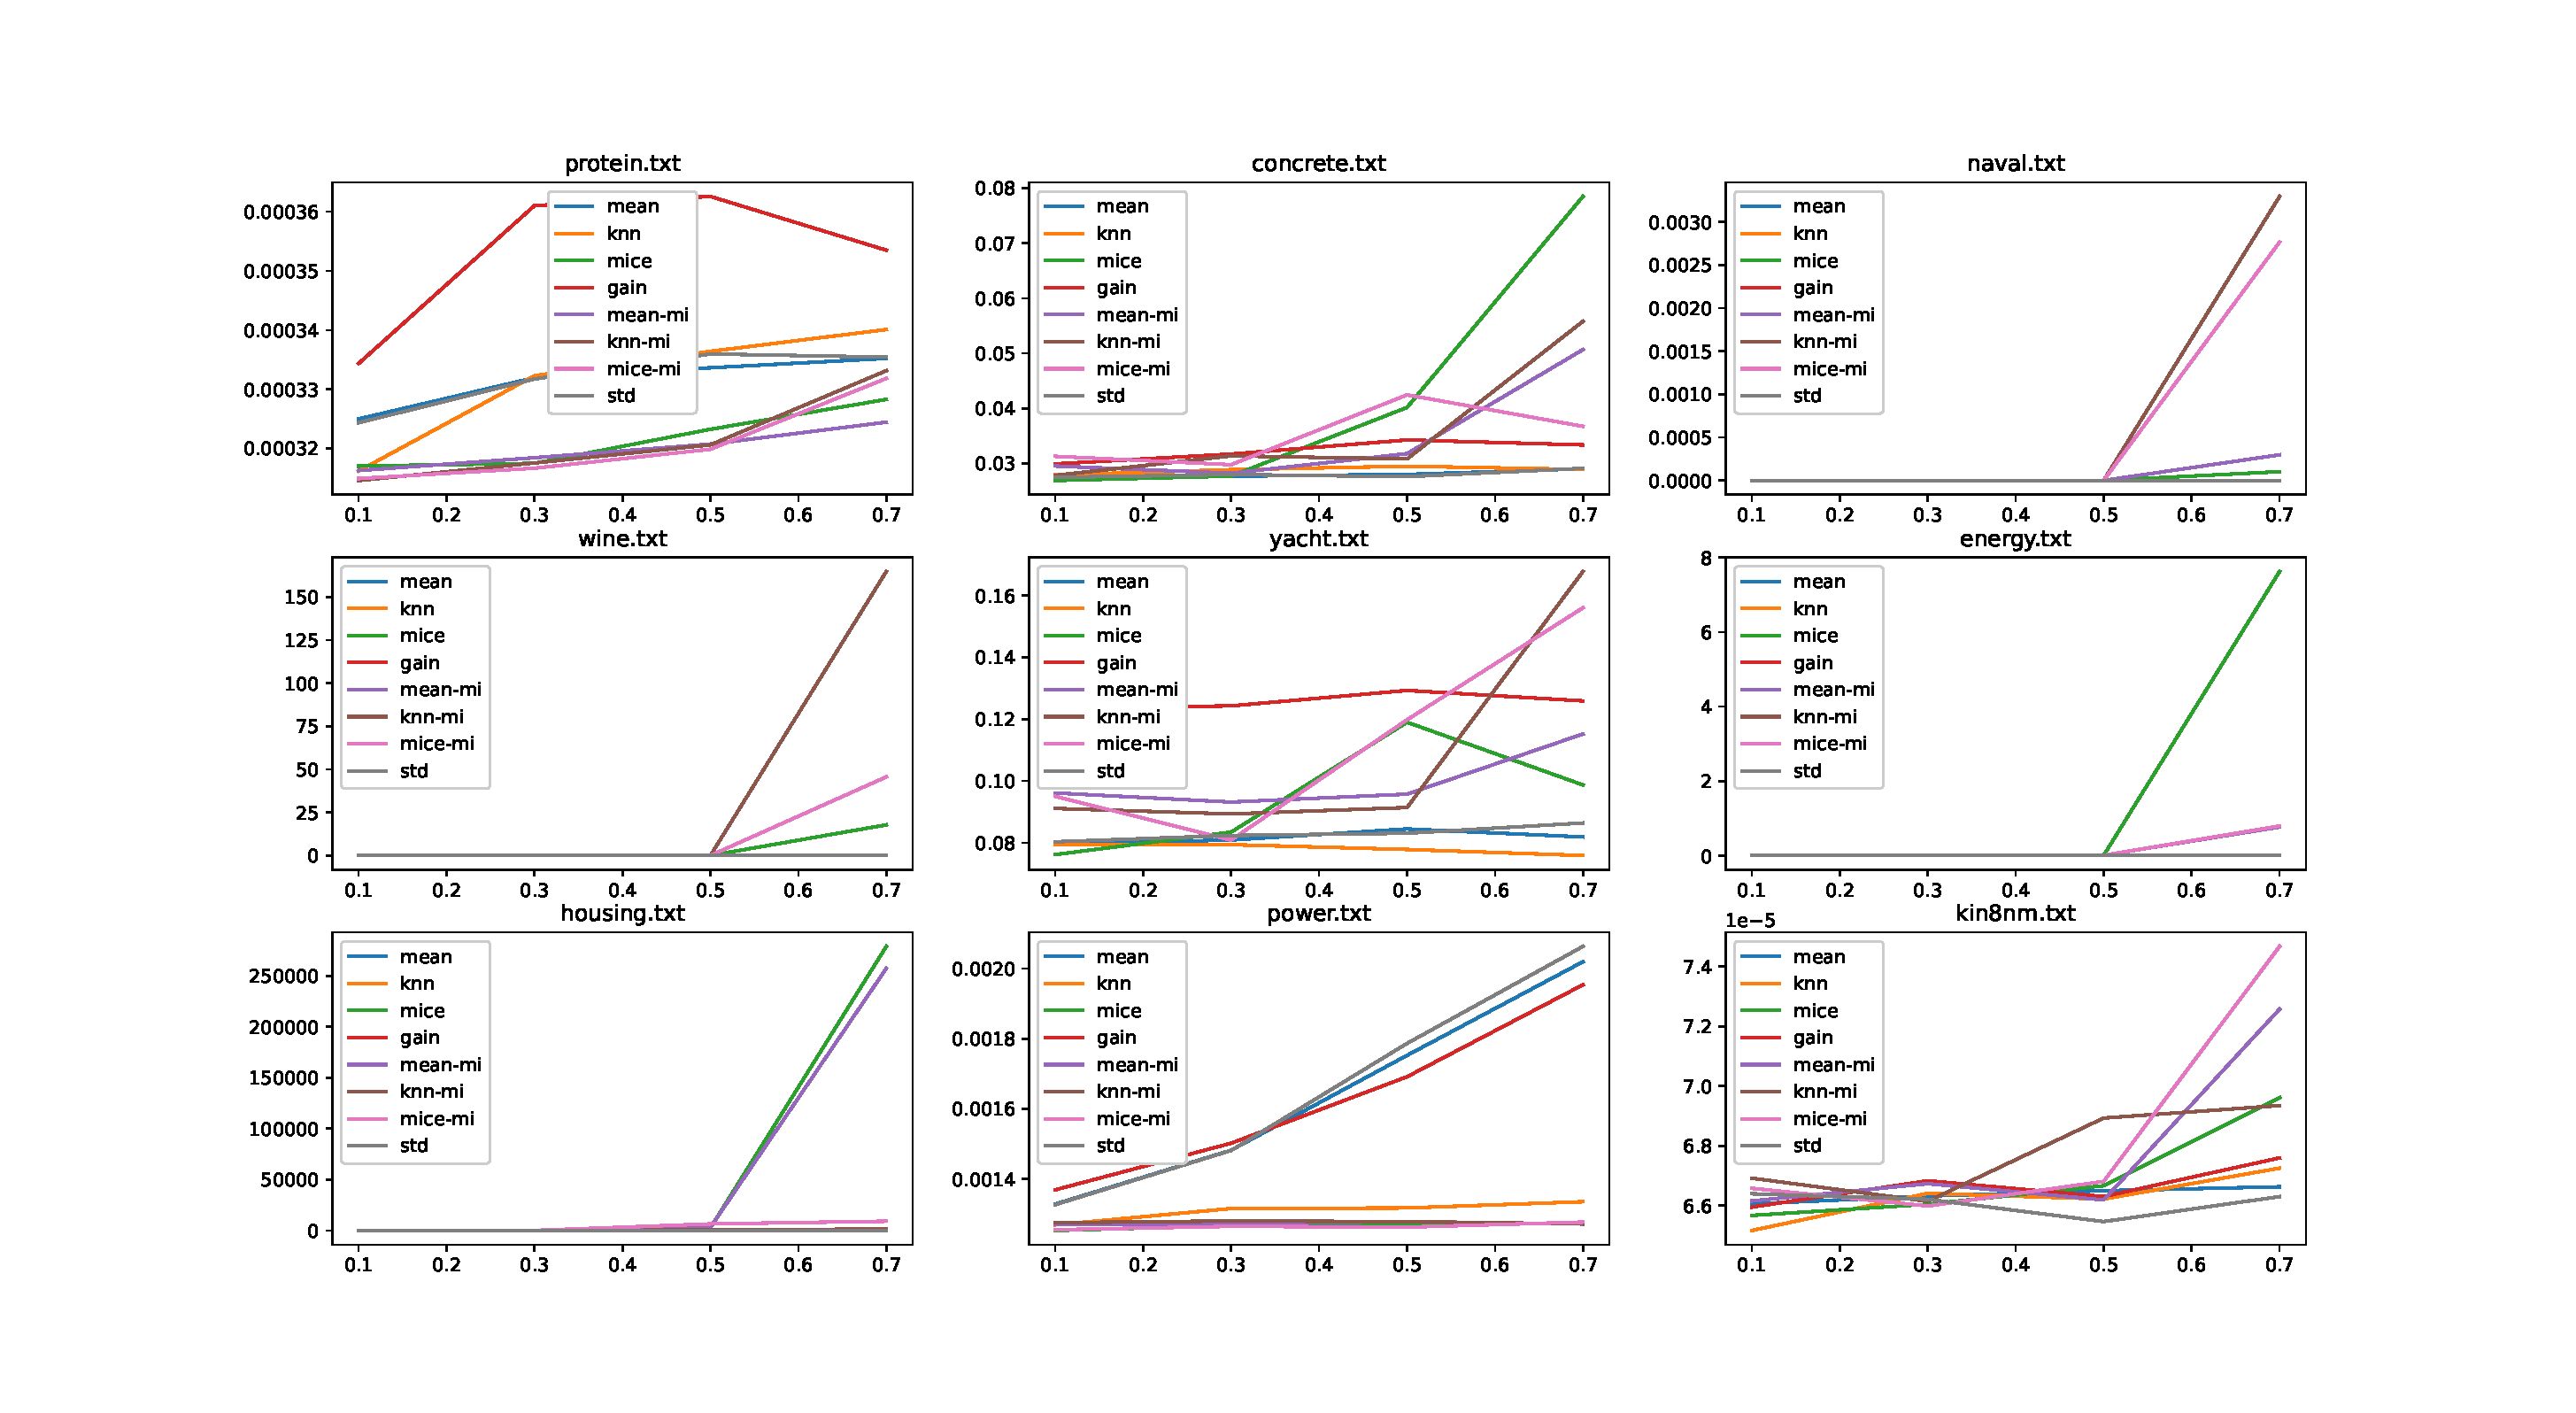
\includegraphics[width=\linewidth]{results_std.eps}
	\caption{Results for uci datasets using different imputation methods
	and different percentages of missing data. The tests cover $0.1, 0.3, 0.5, 0.7$
	probability of missing data. Due to technical difficulties, the GRAPE
	method could not be tested on these sets.}
\end{figure}

%{\small
%\begin{tabular}{|c|c|c|c|c|c|c|c|c|c|}
%	
%	method & protein & concrete & naval & wine & yacht & energy & housing & power & kin8nm  \\
%	\hline
%	mean & 0.000324 & 0.027570 & 00.000002 & 0.001044 & 0.079537 & 0.010275 & 0.022652 & 0.001329 & 0.000066 \\
%	\hline
%	knn & 0.000316 & 0.027899 & 0.000000 & 0.001061 & 0.079552 & 0.009590 & 0.022756 & 0.001270 & 0.000065 \\
%	\hline
%	mice & 0.000317 & 0.026895 & 0.000000 & 0.001033 & 0.076183 & 0.009187 & 0.022649 & 0.001254 & 0.000066 \\
%	\hline
%	gain & 0.000334 & 0.029920 & 0.000002 & 0.001085 & 0.123449 & 0.015222 & 0.024794 & 0.001369 & 0.000066 \\
%	\hline
%	mean-mi & 0.000316 & 0.029528 & 0.000000 & 0.001091 & 0.096109 & 0.010834 & 0.029591 & 0.001270 & 0.000066 \\
%	\hline
%	knn-mi & 0.000314 & 0.027822 & 0.000000 & 0.001124 & 0.091094 & 0.009768 & 0.029503 & 0.001276 & 0.000067 \\
%	\hline
%	mice-mi &0.000314 & 0.031291 & 0.000001 & 0.001098 & 0.095027 & 0.010248 & 0.024455 & 0.001256 & 0.000067 \\
%	\hline
%	std & 0.000324 & 0.027859 & 0.000002 & 0.001080 & 0.078737 & 0.009917 & 0.021778 & 0.001315 & 0.000065 \\
%	\hline
%\end{tabular}
%}
In the energy dataset, similar to the concrete, mice has the largest spike in erorr
after being rougly tied with the other methods.
The most interesting result occurs in the housing dataset, where
mice and mean-mi have the largest error magnitudes of the entire experiment, 
reaching many thousands of times the errors of other methods.
During testing of both these methods, a few of the tests with each $p$ would have low errors,
in line with the other methods, and the next iteration would have a
wildly great error.

The power dataset shows the mean and the gain having the largest error, 
which is the only dataset where the mean behaves so, contrary to our
expectations.
The kin8nm dataset shows the mice-mi and mean-mi datasets with the largest errors.

Considering our method, its error tends to stay among the lowest we tested.
More tests would be required to determine the validity of this simple method.
The smaller the standard deviation, the more this method resembles the
other statistical methods.
This shows that more complex methods are not necessarily the most appropriate
when performing data imputation.
GAIN, which uses a complex adversarial architecture, by no means performed
the best in our experiments.
While that may be a matter of the settings of our test, the extra
time necessary for the imputation (running both generator and discriminator),
does not drastically reduce the erorr over simpler methods.

Besides the error values, the time to perform the imputation can be a large factor
in choosing a specific method.
Since data imputations are usually done as the first part in the pipeline, 
before passing the data to another model, adding even more time to the 
training process in this way might not be feasible.
During our experiments, the gain and $k$nn methods were by far the ones
with the longest imputation time.
As we predicted, calculating the nearest neighbors of each missing value
did indeed make imputation time longer, especially at higher $p$.

The results are included in \texttt{results.txt} since they didn't fit into a single table
on the document.

\section{Conclusions}
In this assignment, we explored several different kinds of imputation methods and (mostly 
successfully) compared their performance on the famous uci datasets.
While we tested statistical and deep approaches, there are still different 
types, such as matrix factorization methods, that we did not get the 
chance to test.
We then slightly tweaked an existing method to come up with a method
based on the standard deviation of the observed feature values.

Feature imputation is a very important step in the data collection and
preprocessing steps.
Imputation itself is a precursor to actually training a model.
While models can take a long time to train, we may not want our 
imputation to also take much time or resources, since our data might
be changing or growing constantly.

Some of the imputation methods we tested used simple statistical proerties
of the data to impute values, such as  the mean or standard deviation, 
while others used clustering and even deep learning based approaches.
While each has their strengths and weaknesses, we ultimately want
a method that is suitable for our use case.
Some use caess might not allow ``good enough'' results and require
the lowest possible errors, while other use cases might be more 
concerned with getting an acceptable data up and running.

One of our takeaways from this assignment is that, at least on these
simple datasets, simpler methods do not necessarily outcompete 
complex ones.
The mean, which we thought beforehand would have the worst performance,
showed to be an acceptable choice in different datasets.
Going forward, those wanting to train models should pay more attention
to the quality of the data and how it gets preprocessed.


Future work in this area could include simpler methods that utilize
some other property of the data, similar to our std aproach here.
The models we use here assume the data is collected i.i.d.
It would not make sense to use the mean or standard deviation
unless samples were drawn from similar distributions.
However, in recent years there has been research into scenarios where
the data is imbalanced~\cite{he2009learning}, when samples do not resemble each other or 
violate the i.i.d.\ assumption.
A model which could be useful in scenarios where traditional methods
have not gone.

Many people pay little attention to the imputation methods used,
and while in our experiments the difference was not very large most of the time
the error in some cases would be disastrous to any project.
A better understanding of which types of cases are better suited to each 
approach, combined with experimentation, could greatly help in 
the pre-processing step.
\printbibliography
\end{document}
